%% 美赛模板:正文部分
\documentclass[12pt]{article}  % 官方要求字号不小于 12 号,此处选择 12 号字体
% 本模板不需要填写年份,以当前电脑时间自动生成
% 请在以下的方括号中填写队伍控制号
\usepackage[2012050]{easymcm}  % 载入 EasyMCM 模板文件
\problem{C}  % 请在此处填写题号
\usepackage{mathptmx}  % 这是 Times 字体,中规中矩 
%\usepackage{mathpazo}  % 这是 COMAP 官方杂志采用的更好看的 Palatino 字体,可替代以上的 mathptmx 宏包

\usepackage{threeparttable}    %这行要添加
\usepackage{verbatimbox}

% 算法排版
\let\algorithm\relax
\let\endalgorithm\relax
\usepackage[linesnumbered,ruled,vlined]{algorithm2e}%[ruled,vlined]{
\usepackage{algpseudocode}
\usepackage{amsmath}
\renewcommand{\algorithmicrequire}{\textbf{Input:}}
\renewcommand{\algorithmicensure}{\textbf{Output:}}

\usepackage{xcolor} % 定制颜色
\definecolor{mygreen}{rgb}{0.15,0.66,0.7}
\definecolor{myblue}{rgb}{0,0,164}
\definecolor{mygray}{rgb}{0.6,0.65,0.74}
\definecolor{mymauve}{rgb}{0.58,0,0.82}

\lstset{
	numbers=left, 
	breaklines=true,              
	columns=fixed, 
	commentstyle=\color{mygray}\rmfamily\itshape,    
	keywordstyle=\color{myblue},    
	stringstyle=\color{mygreen}\ttfamily,  
	rulesepcolor=\color{red!20!green!20!blue!20} }


\title{ Data Analysis on Product Review System: A Comprehensive Evaluation Model}  % 标题

\bibliographystyle{unsrt} % BibTex

% 如需要修改题头(默认为 MCM/ICM),请使用以下命令(此处修改为 MCM)
%\renewcommand{\contest}{MCM}

% 文档开始
\begin{document}

% 此处填写摘要内容
\begin{abstract} 
\setlength{\parskip}{1em}
E-commerce is growing at an unprecedented rate all over the world. In the process of purchasing goods, ratings and reviews play a vital reference role. Companies are pursuing a comprehensive and understandable analysis of online market data to craft greater success.

In this paper, we seek to devise several approaches to analyze the product evaluation by exploring ratings, text-based reviews and other related indicators.

We first perform exploratory data analysis by generating the data quality report and studying the distribution of the most critical indicators. Then we preprocess reviews by a series of steps, including removing punctuations, converting abbreviations, etc. Besides, we extract the frequent features of each product using \textbf{WordCloud}.

We then build PRMP, a framework that defines the patterns, relationships, measures, and parameters within and between ratings and reviews. We use \textbf{SentiWordNet} to obtain the sentiment of a review and normalize star ratings and helpfulness. Through \textbf{association analysis}, we visualize the relationship using a set of heat maps and draw conclusions from them.  

After that, we propose a new approach to find a traceable measure for the product. We use \textbf{Entropy Weight Method} to obtain weights of the indicators. To identify reputation trends over time, we use the \textbf{ARIMA Model} to fit the reputation score. We select one of the hair dryer products as our main study object, calculate its score over time and give its most likely trending result.  We use the \textbf{Non-linear Programming Model} to find the best combination of text-based and rating-based measures to indicate potential success and failure. We apply the \textbf{Hovland Persuasion Model} to build a decision model that describes the indicators that influence customer decisions, achieving the combination of the theory of social psychology and real-life context. And to analyze specific quality descriptors, we classify words into eight categories using the \textbf{NRC Emotion Lexicon}. Then we match the emotional intensity with star ratings and find the relationship between them.

Finally, based on the established model and detailed analysis, we put forward practical suggestions for Sunshine Company's marketing plan to improve its product competitiveness.

	
	
	% 美赛论文中无需注明关键字。若您一定要使用,
	% 请将以下两行的注释号 '%' 去除,以使其生效
	% \vspace{5pt}
	% \textbf{Keywords}: MATLAB, mathematics, LaTeX.

\end{abstract}



		% 摘要请到ABSTRACT.tex中填写

\maketitle  % 生成 Summary Sheet
\tableofcontents  % 生成目录


% 正文开始
\section{Introduction}
\subsection{Background}
Globally, more than 50\% of e-commerce sales were made through online marketplaces in 2019, contributing \$1.7 trillion to the economy each year.[1] E-commerce is growing at an unprecedented rate. Amazon, as the top online marketplace, provides customers with an opportunity to review products and express their level of satisfaction by rating. At the same time, ratings and reviews can reduce potential annoyance on the buying experience. 


Companies use these data to analyze the market demand, the timing of market participation, and product optimization. The description and evaluations of products are one of the most valuable references to customers when shopping online. An analysis of ratings and reviews for similar products from Amazon is critical to the company's sales strategies and can help increase product competitiveness. 


\subsection{Problem Restatement and Our Work}
Sunshine Company is planning to introduce and sell three new products in the online marketplace. Therefore, online sales strategy, analysis of product reviews are needed to craft success in the future.

We are provided with data on ratings, reviews for microwave ovens, baby pacifiers and hairdryers sold in Amazon in recent years. 

In this paper, we broke our work into sections as follows.
\begin{enumerate}[\bfseries 1.]
    \item  We analyze the three data sets thoroughly and generate the data quality report.
    
    
    \item  We preprocess text-based reviews to fit our natural language processing model better.
    
    
    \item  We use SentiWordNet to obtain the sentiment of the review and then find the relationships between and within star ratings, reviews, and helpfulness ratings.
    
    
    \item  Based on the product evaluation on Amazon, we create measures to analyze the reputation of a product and used the ARIMA model to see how it changes over time.
    
    \item We use a non-linear programming model to explore the combinations of dimensions that best indicate a potentially successful or failing product.
    
    
    \item  Applying Hovland Persuasion Model, we perform a decision analysis on motivation for a person to change a review.
    
    
    \item To analyze specific quality descriptors, we use the NRC Emotion Lexicon to obtain the intensity of eight categories of word sentiment, including anger, fear, trust, etc. Then we match the emotional intensity with star ratings to see if they were somehow related. 
    
    
    \item  Finally, based on the established model and detailed analysis, we put forward practical suggestions for Sunshine Company's marketing director to improve their product competitiveness.
    
   
    
\end{enumerate}

\section{Assumption and Data Exploration}
\subsection{Assumption}
\begin{itemize}
	\item The product evaluations are all reasonable. That is, there is no extreme situation like low star rating and great review. We found it rare when checking the dataset.
	
	
\end{itemize}

\subsection{Data Quality Report}
The data quality report is the most important tool of the data exploration process. The tabular reports are accompanied by data visualizations that illustrate the distribution of the values in each feature in an \textbf{ABT}(analytical base table)\cite{kelleher2015fundamentals}.

Data quality report of \textbf{hair\_dryer.tsv} is shown as \textbf{Table \ref{tb:abt}}.
\begin{table}[!htbp]
	\begin{center}
		\caption{Analytical Base Table}\label{tb:abt}
		 \begin{threeparttable}      
		 	\addvbuffer[12pt -18pt]{    %这行要添加
			\begin{tabular}{ccccccc}
			\toprule
			%	\multicolumn{3}{c}{test}\\
			%	\midrule
			\multicolumn{1}{m{2cm}}{\centering }
			&\multicolumn{1}{m{3cm}}{\centering customer\_id}
			&\multicolumn{1}{m{3cm}}{\centering product\_parent}
				&\multicolumn{1}{m{2cm}}{\centering star\_rating}
			&\multicolumn{1}{m{2cm}}{\centering helpful\_votes}
				&\multicolumn{1}{m{2cm}}{\centering total\_votes}\\
			\midrule
			$Count$&11470.00&11470.00&11470&11470&11470\\
			$Mean$&28151220.00&484633800.00&4.116042&2.179076&2.563296\\
			$Std$ &152387700.00&287324000.00&1.300333&14.241304&15.38258\\
			$Min$ &12464.00&42396.00&1&0&0\\
			$Lower\; Quartile$ &14914410.00&235106000.00&4&0&0\\
			$Media$ &27071230.00&486774000.00&4&0&0\\
			$Upper\; Quartile$ &42336440.00&732252300.00&5&1&1\\
			$Max$ &53096370.00&999436600.00&5&499&575\\
			\bottomrule
			\end{tabular}}
        %这行要添加
		\end{threeparttable}       %这行要添加,到这里结束
	\end{center}
\end{table}


From this report, it is clear that there is no continuous values are missing, so there is no need to fit any missing values. Star\_rating is quite skewed and mostly concentrated on the 5. Meanwhile, there are also some extreme values in \textsl{`helpful\_votes'} and \textsl{`total\_votes'} that are worth exploring.

All data reports from the three data sets are similar, so we won't go into details here.

\subsection{Review Preprocessing}
For the categorical features, we selected four main features which are `vine', `verified\_purchase', `review\_headline' and `review\_headline' as our main targets. The first two are essentially boolean values but `review\_headline' and `review\_body' are long strings and need to be modified.

Here are our preprocessing steps for `review\_headline' and `review\_body':


\begin{enumerate}[\bfseries 1.]

	\item Begin by removing dirty strings in the reviews, such as html tag `<br>'.
	
	\item Convert English abbreviations to full expressions, such as changing `isn't' into `is not'.
	
	\item Remove any punctuations, alpha-numeric and any other words in the limited set of special characters like `', or `.' or `\#' etc.
	
	\item Cut a sentense into seperate words, remove stopwords and convert the remain words to lowercase.
	
	\item When processing review headlines, add a noun after each word in case the part of speech is misjudge .

\end{enumerate}

\subsection{Preliminary Insights Into the Data}

\textbf{Star Rating.}After our statistical analysis, we can find that the 5-star ratings of the three categories of products are all in the majority. But the difference is that the star rating of the microwave oven product is polarized to 1 star and 5 stars. To avoid the potential extremes that may occur in a small number of evaluations, we selected MICROWAVE as a test target for our models.

\begin{figure}[h]
	\centering
	\begin{subfigure}[b]{.32\textwidth}
		\centering
		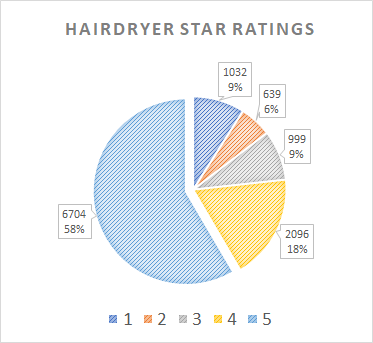
\includegraphics[scale=0.38]{star_HAIRDRYER.png}
		\caption{Star Distribution of Hair dryer }
	\end{subfigure}
	\begin{subfigure}[b]{.32\textwidth}
		\centering
		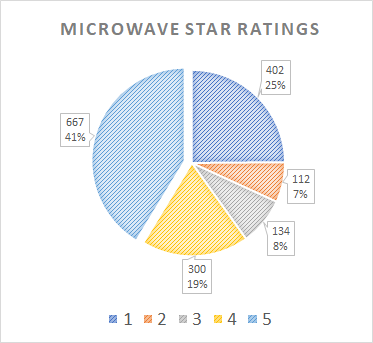
\includegraphics[scale=0.38]{star_MICROWAVE.png}
		\caption{Star Distribution of Microwave}
	\end{subfigure}	
	\begin{subfigure}[b]{.32\textwidth}
		\centering
		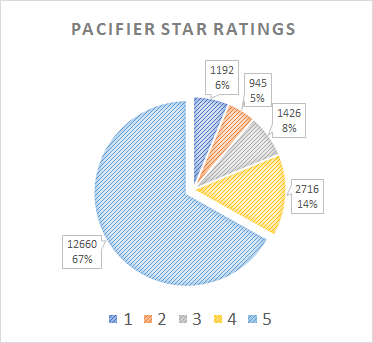
\includegraphics[scale=0.38]{star_PACIFIER.png}
		\caption{Star Distribution of Pacifier}
	\end{subfigure}	
	\caption{Star Distribution of Each Product}
	\label{fig:fig1}
\end{figure}

\textbf{Review.}From the reviews of the three products, we can find the adjective words sifted by WordCloud. The first words that catch the eye are 'great', 'good', 'little' and 'new', then the adjective words related to the specific product. We also generate the feature word cloud of each product in the letter to Sunshine Company.

\begin{figure}[h]
	\centering
	\begin{subfigure}[b]{.32\textwidth}
		\centering
		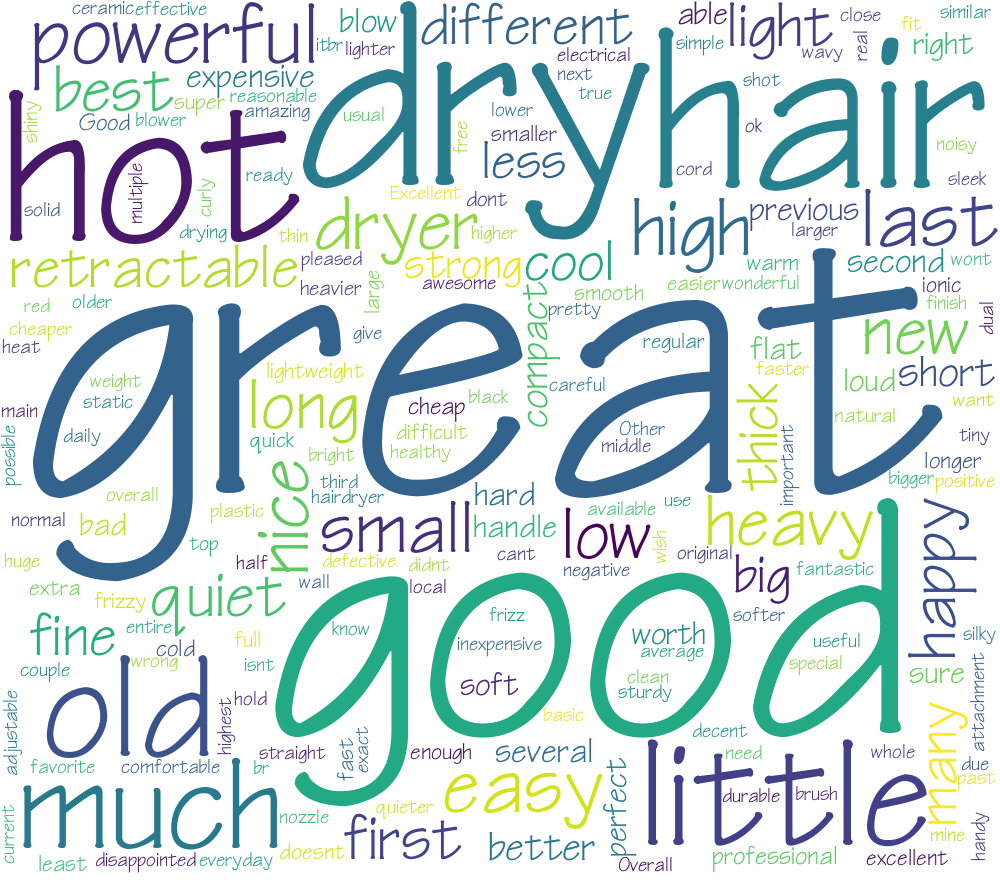
\includegraphics[scale=0.125]{wordcloud_hairdryer.png}
		\caption{Review Wordcloud of Hair dryer}
	\end{subfigure}
	\begin{subfigure}[b]{.32\textwidth}
		\centering
		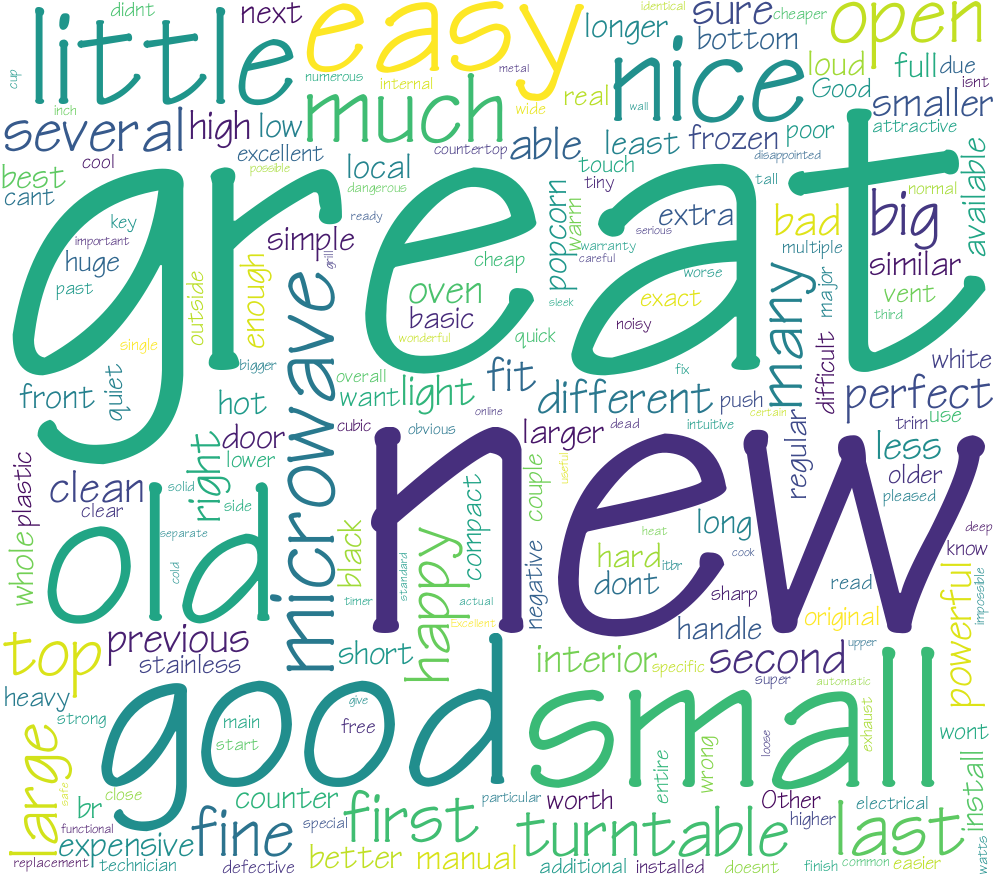
\includegraphics[scale=0.125]{wordcloud_microwave.png}
		\caption{Review Worcloud of Microwave}
	\end{subfigure}	
	\begin{subfigure}[b]{.32\textwidth}
		\centering
		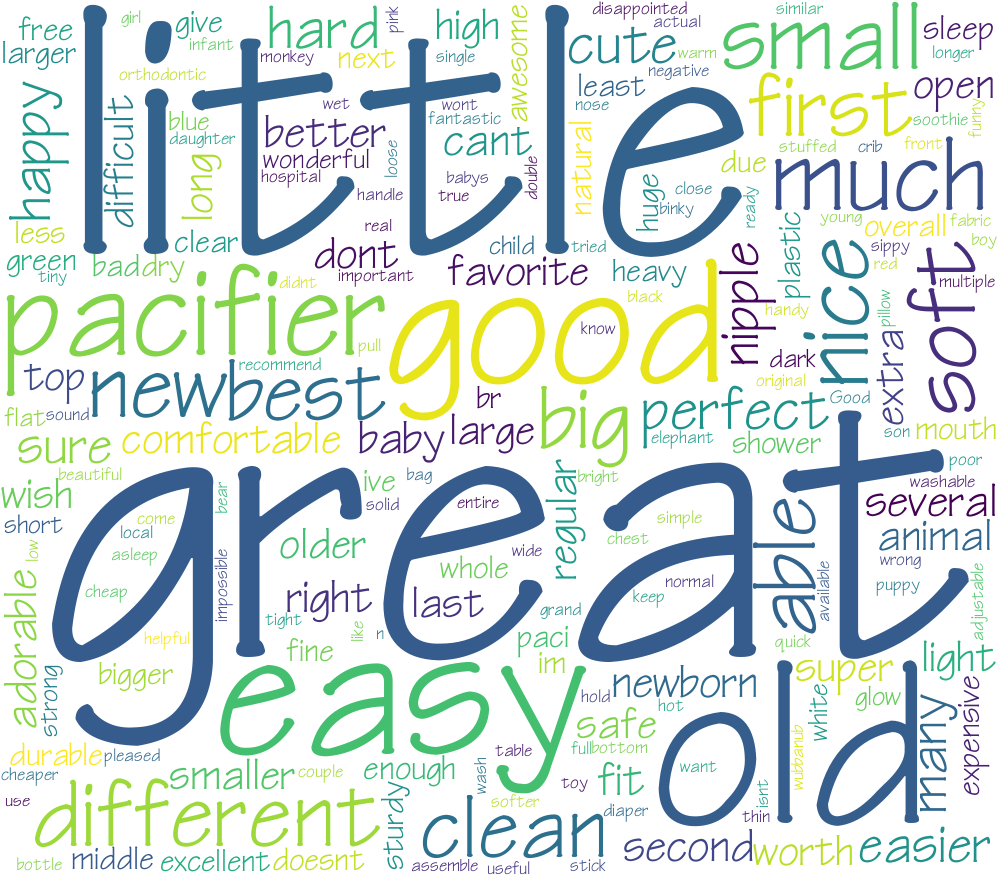
\includegraphics[scale=0.125]{wordcloud_pacifier.png}
		\caption{Review Wordcloud of Pacifier}
	\end{subfigure}	
	\caption{Review Wordcloud of Each Product}
	\label{fig:fig2}
\end{figure}


\section{PRMP Model}
The evaluation of a product has a significant impact on whether other customers purchase the product. Star ratings, reviews, and helpfulness ratings are the most valuable references to customers when shopping online, so we consider them as our primary measure factors.

\subsection{Review}
\subsubsection{Sentiment}
To analyze customer reviews, we mainly focused on analyzing opinions in the reviews and categorizing the reviews into positive or negative based on customer sentiment.

\textbf{SentiWordNet}\cite{baccianella-etal-2010-sentiwordnet} is the result of the automatic annotation of all the synsets of WORDNET according to the notions of ``positivity'', ``negativity'', and ``neutralit''. Each synset s is associated to three numerical scores Pos(s), Neg(s), and Obj(s) which indicate how positive, negative, and ``objective'' (i.e., neutral) the terms contained in the synset are.[baccianella-etal-2010-sentiwordnet]

We found whether a review is positive or negative in the following steps:

\begin{enumerate}
	\item[1.)] Preprocessing reviews using methods shown in section 2.3 and extract 
	adjectives and coordinating conjunctions, which reveal more emotions and opinions of review.
	
	\item[2.)] Using the SentiWordNet to find the positive and negative values related to each word in a review and consider the impact of its neighboring words.
	
	\item[3.)] Summing up the obtained positive and negative values to calculate a net positive and net negative values related to a review.
	
\end{enumerate}

\begin{figure}[!htbp]
	\centering
	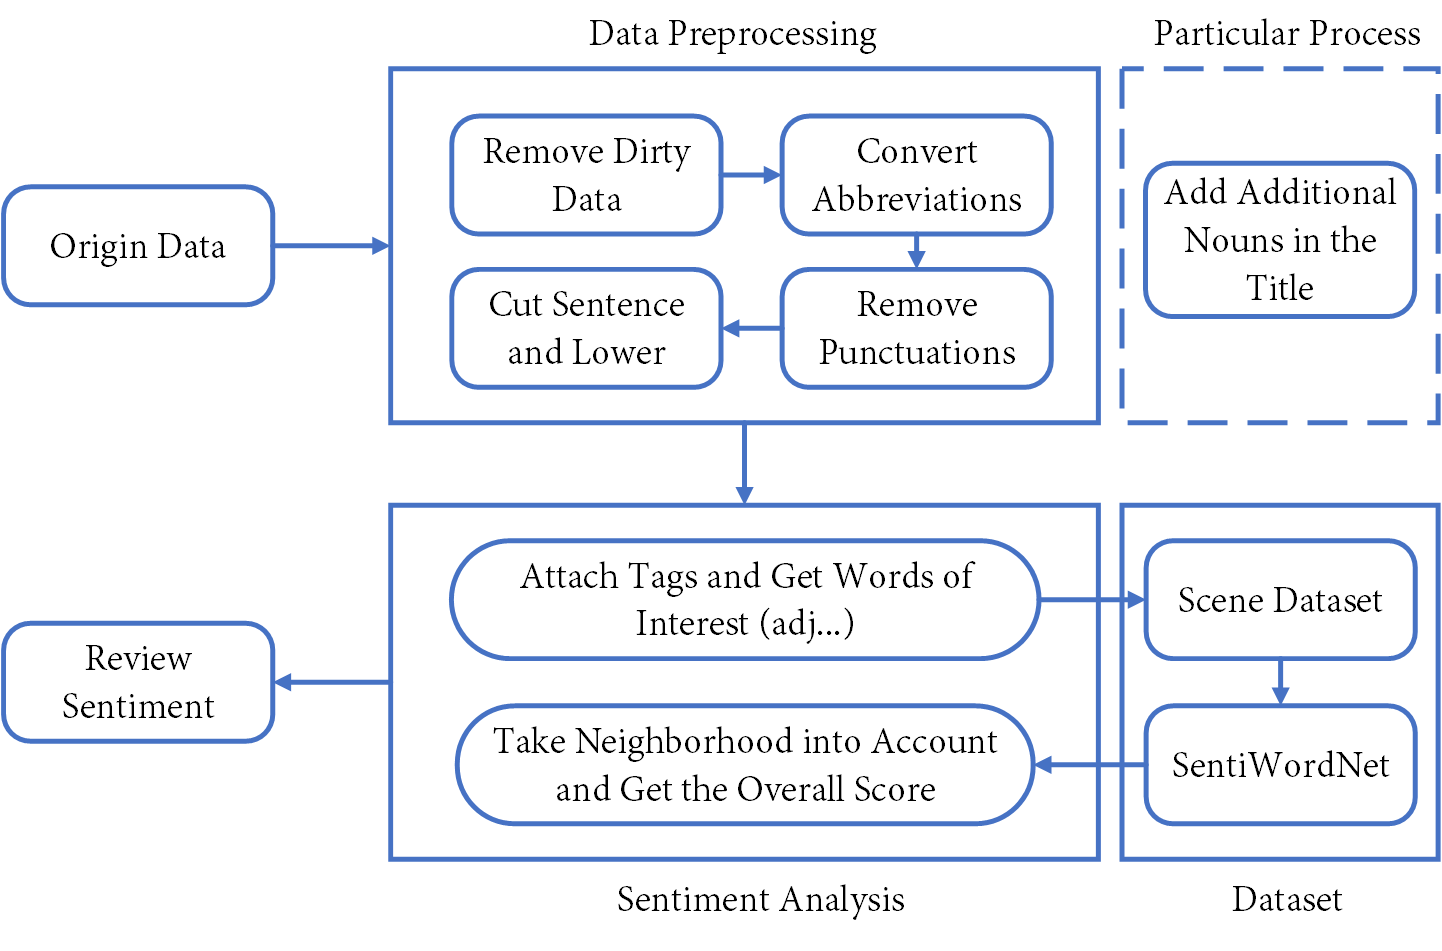
\includegraphics[scale=0.5]{process.png}
	\caption{Flowchart of the Sentiment Processing}
	\label{fig:fig3}
\end{figure}

The sentiment of a review results in [-1, 1], and we normalize it so that the result is between 0 and 1.


\subsubsection{Readability and Length}

Readability and length of the text are a direct expression of the intelligibility of the review text. In other words, intelligibility is judged by the difficulty of reading and understanding the relevant text.

The more understandable the review is, the more valuable it is. Therefore, intelligibility can be theoreticalized at the cognitive level, based on the cognitive adaptability of the review text to ordinary consumers.

Readability tests have been used to study the quality characteristics of several types of text in different areas of information science, and a number of readability indicators have been developed over the years. We cite the following two quantitative criteria: The Fog index measure complexity, and the ARI index measure reading ease\cite{KorfiatisEvaluating}.  

\begin{equation}
	FOG = 0.4\times(\frac{Words}{Sentence}+100\times(\frac{N(complex\_words)}{N(words)}))
\end{equation}

\begin{equation}
ARI = 4.71 \times (\frac{characters}{words})+0.5\times(\frac{words}{sentence})-21.43
\end{equation}

Based on these, a quantitative study on the readability of text can be carried out. Due to the limited space of the article, we will not expand the description.

\subsection{Star Rating}
Star ratings tell people the quality of the product in an intuitive way, which may have an impact on customers' decisions. In general, a moderate star rating(like three stars) shows customers' neutral attitude and gives little information. What customers pay attention to are the extreme star ratings, which can convey more information.

Star ratings are originally a set of integers from 1 to 5. To better fit our model, we performed normalization on it. 

\begin{table}[!htbp]
	\begin{center}
		\caption{Star Normalized Value Table}%\label{tb:abt}
		\begin{threeparttable}      
			\addvbuffer[12pt -18pt]{    %这行要添加
				\begin{tabular}{cccccc}
					\toprule
					%	\multicolumn{3}{c}{test}\\
					%	\midrule
					\multicolumn{1}{m{3cm}}{\centering star\_ratings}
					&\multicolumn{1}{m{2cm}}{\centering 1}
					&\multicolumn{1}{m{2cm}}{\centering 2}
					&\multicolumn{1}{m{2cm}}{\centering 3}
					&\multicolumn{1}{m{2cm}}{\centering 4}
					&\multicolumn{1}{m{2cm}}{\centering 5}
					\\
					\midrule
					after normalization&0&0.25&0.5&0.75&1\\
					\bottomrule
			\end{tabular}}
			%这行要添加
		\end{threeparttable}       %这行要添加,到这里结束
	\end{center}
\end{table}
\subsection{Helpfulness}
Counting helpful votes is a measure of the quality of a review. With a certain total number of votes, the more helpful votes a review receives from other customers, the more valuable the review is.

We define the \textbf{Helpful Votes Ratio} of a review (\textbf{HVR}) as the number of helpful votes a review gets divided by the total number of votes.
\begin{equation}
HVR=\frac{helpful \; votes}{total \; votes}
\end{equation}

If a review doesn't receive any votes at all, we define its HVR as 0.5, which means that this review was neither helpful nor unhelpful.


\subsection{PRMP Model and Result}

We propose a \textbf{PRMP} model that defines the patterns, relationships, measures, and parameters within and between star ratings, reviews, and helpfulness ratings.


\begin{figure}[!htbp]
	\centering
	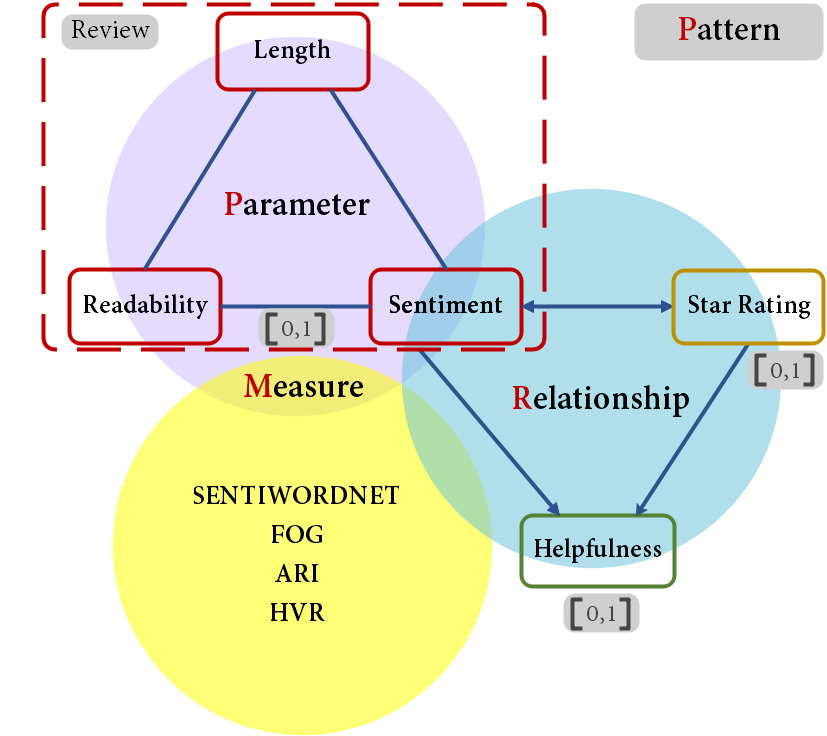
\includegraphics[scale=0.5]{relationship.png}
	\caption{The Concept Graph of PRMP Model}
	\label{fig:fig4}
\end{figure}

Through the association analysis, we drew the following heat map. Star rating is closely related to the sentiment of a review and has an almost linear correlation. 

\begin{figure}[htbp]
	\centering
	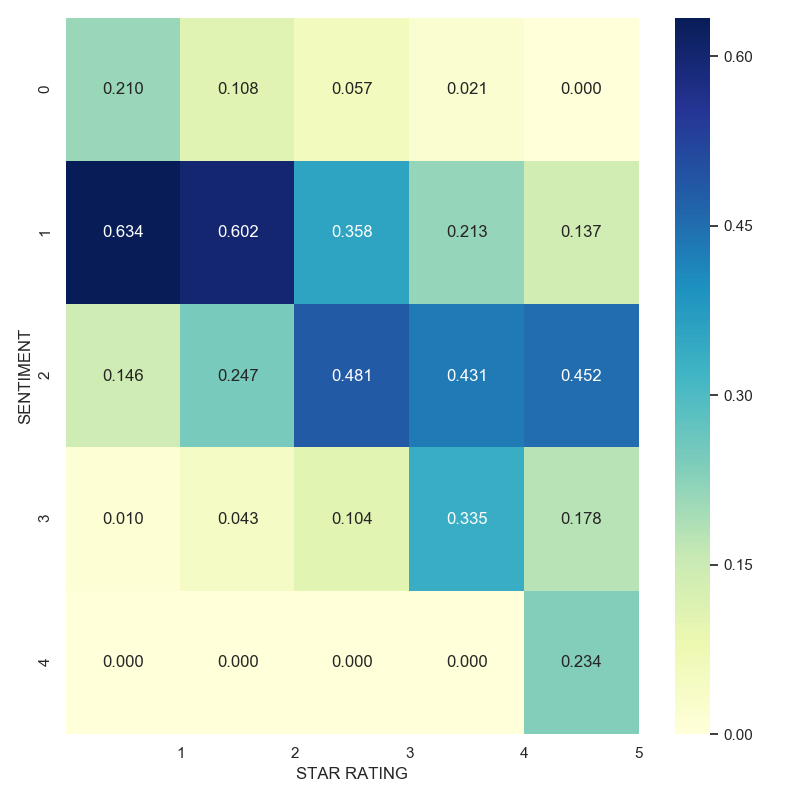
\includegraphics[scale=0.3]{07.png}
	\caption{The Correlation Between Sentiment and Star Rating}\label{fig:fig5}
\end{figure}

The dark areas other than the diagonal in the heat map may have something to do with parameter adjustment.

When we performed the association analysis with helpfulness, we got different results. From the two heat maps below, the helpfulness and the other two parameters do not seem to be directly related. However, it is worth noting that in the helpfulness and star rating heat map, 1-star reviews seem to get more support from others than 5-star reviews. Low star reviews may be more helpful because of illustrating the actual problems with the product.

\begin{figure}[h]
	\centering
	\begin{subfigure}[b]{.45\textwidth}
		\centering
		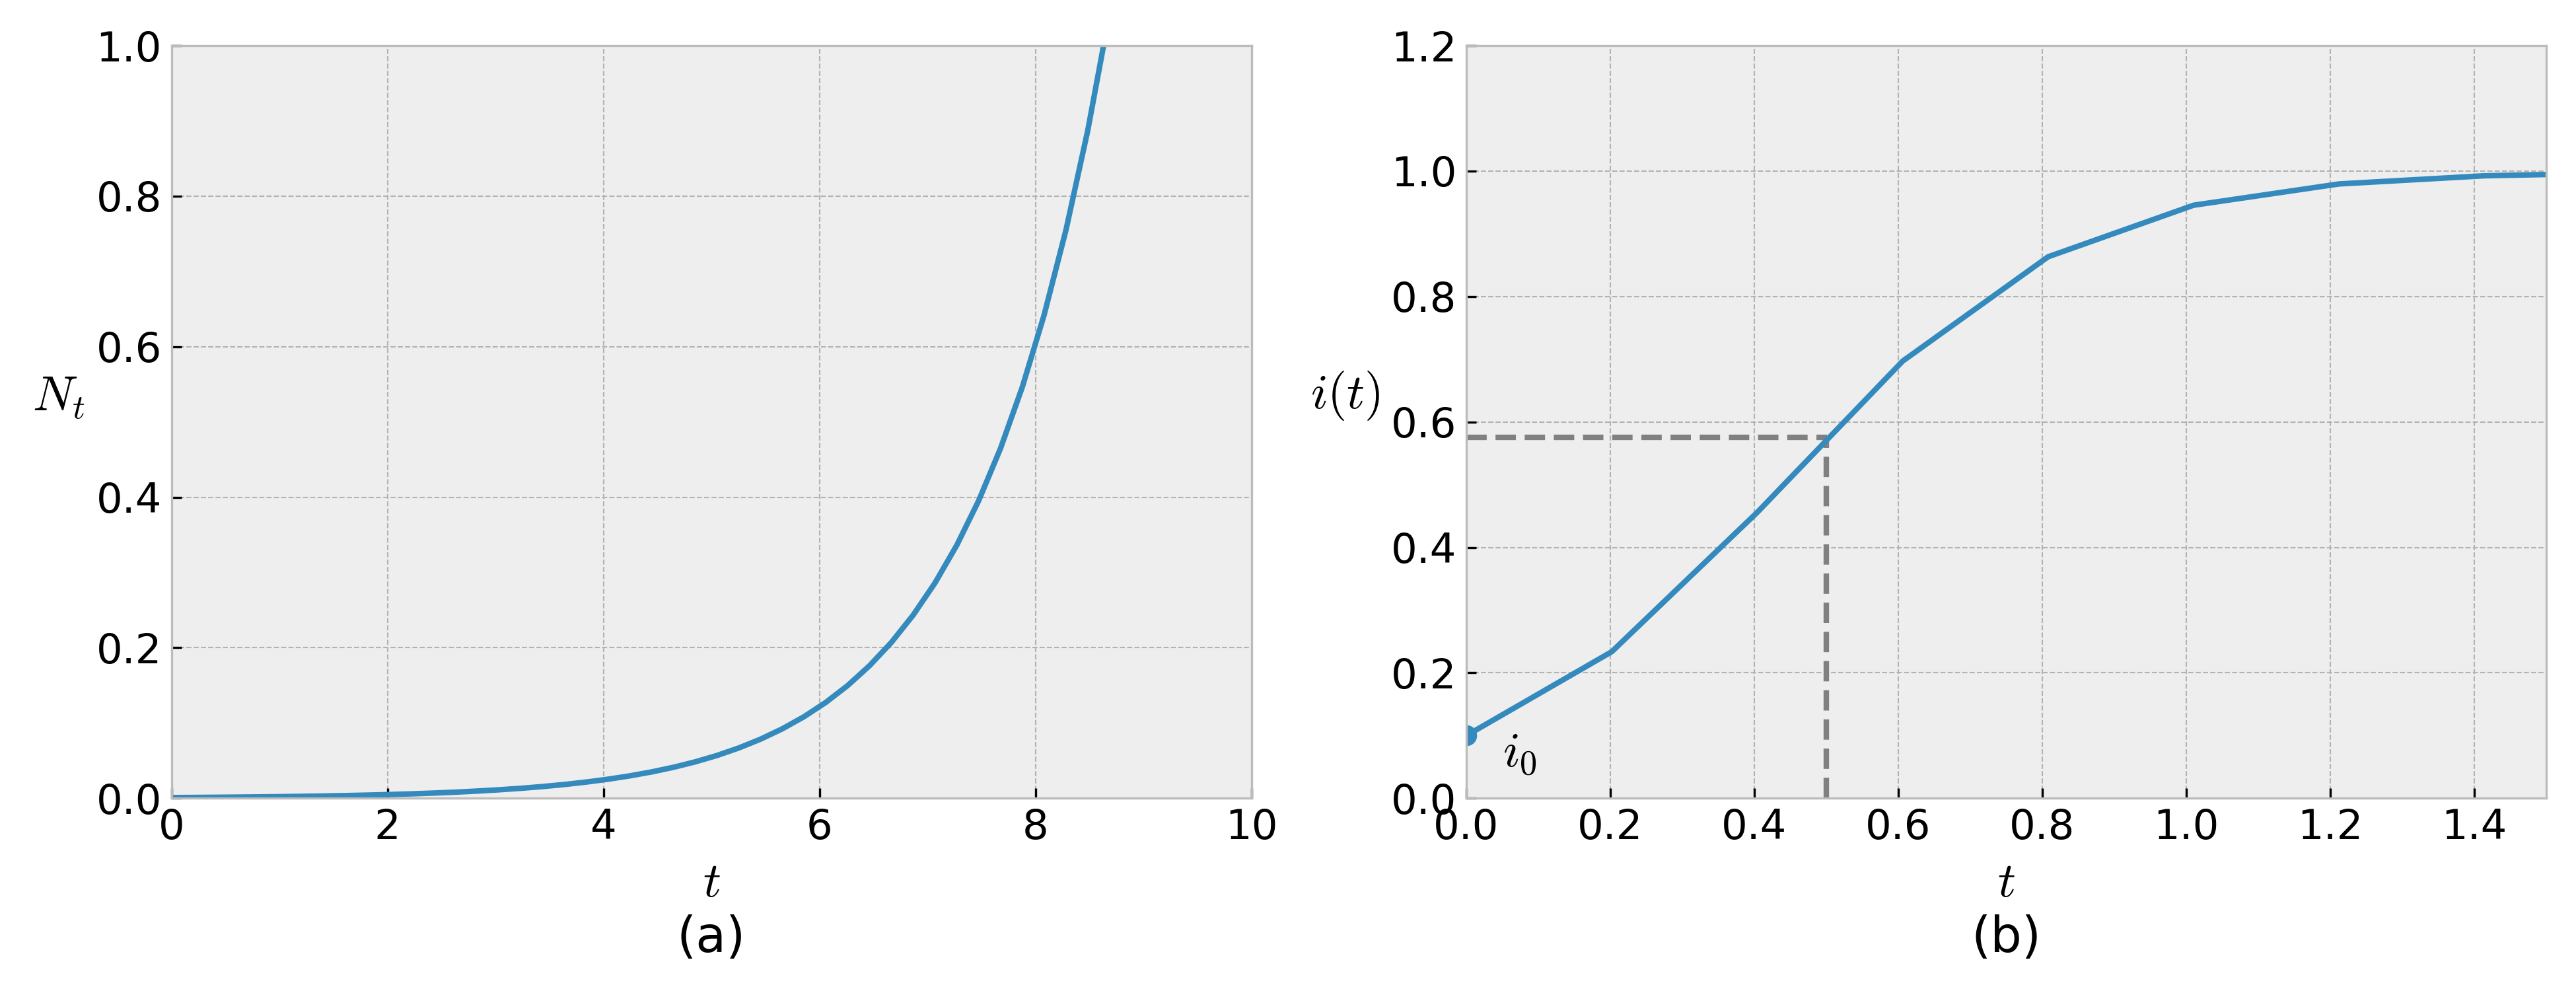
\includegraphics[scale=0.4]{1.png}
		\caption{The Correlation Between Helpfullness and Star Rating}
	\end{subfigure}
	\begin{subfigure}[b]{.45\textwidth}
		\centering
		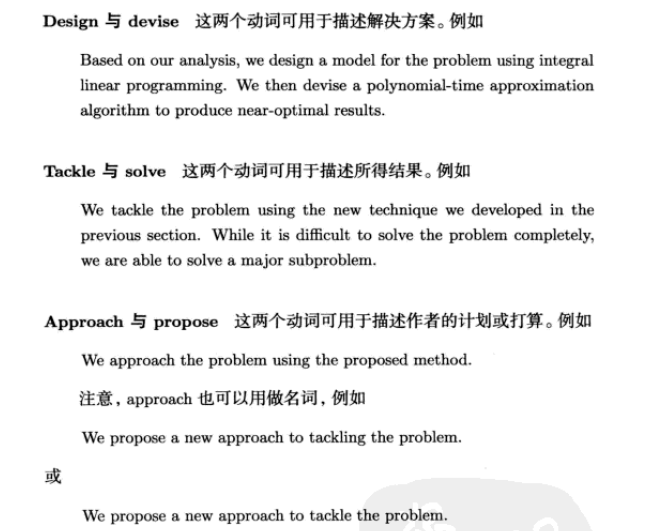
\includegraphics[scale=0.4]{2.png}
		\caption{The Correlation Between Helpfullness and Star Sentiment}
	\end{subfigure}	
	\caption{The Correlation Between Analysis}
	\label{fig:fig6}
\end{figure}

Note: the reason why moderate helpfulness is the majority is that most reviews don't have any votes, so HVR equals 0.5.


\section{Comprehensive Product Evaluation Model}
\subsection{Product Measurement}

We believe that ratings and reviews give different amounts of information. By calculating the respective information entropy and assigning different weights, we get a score of a single product review.

But are all reviews equally important? Our conclusion is no. The importance of a review is also related to its helpfulness and authority. We used HVR to define the helpfulness and assign different weights for various combinations of `vine' and `verified', thus setting the authority.

Considering a star rating and a review can be potentially extreme, we cannot use one evaluation to judge the quality of a product. A short term overall score is needed for Sunshine Company to track.

The figure \ref{fig:fig7} shows our product measure model .


\begin{figure}[htbp]
	\centering
	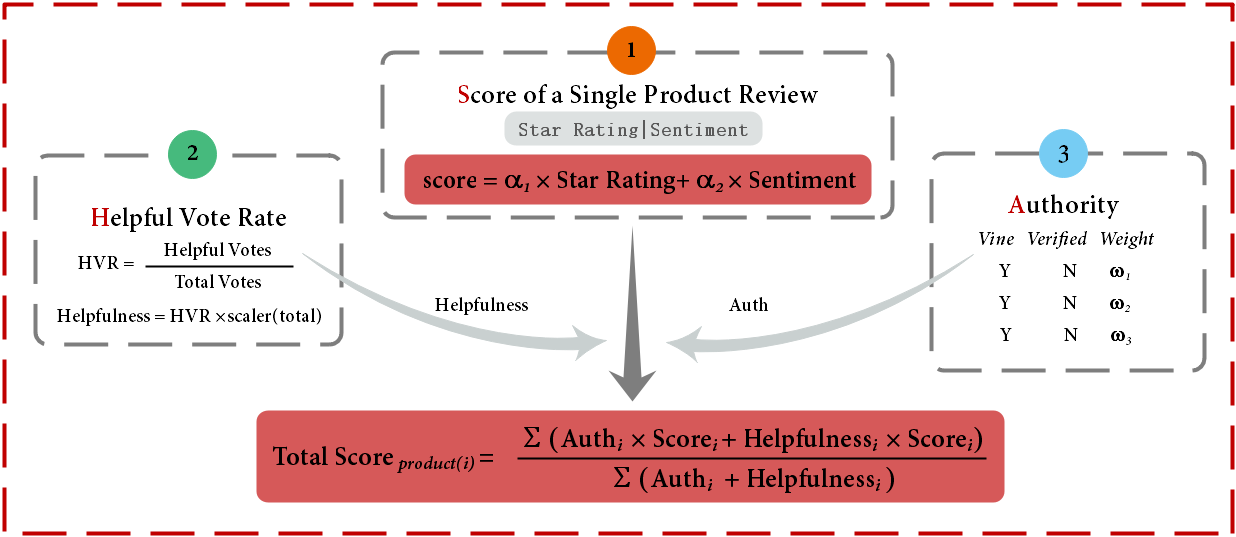
\includegraphics[width=1\textwidth]{model1.png}
	\caption{The Concept Graph of Product Measure Model}\label{fig:fig7}
\end{figure}

\newpage
Since we used indicators with different units, normalization is needed to scale all values in the range [0,1]. Equation\ref{eq:min_max} gives the form of data normalization.

\begin{equation}\label{eq:min_max}
x_{new}=\frac{x-x_{min}}{x_{max}-x_{min}}
\end{equation}

Where $x_{max}$ and $x_{min}$ are the maximum and minimum values of the indicator in the same unit.

\subsubsection{Entropy Weight Method to Obtain $\alpha_1$ and $\alpha_2$}

The weights of star rating and review sentiment are given using the entropy weight method.

According to the definition of information entropy in information theory, the information entropy $E_j$ is equal to:

\begin{equation}\label{eq:entropy}
E_j =-\frac{1}{ln(x)}\sum\limits_{i=1}^{n}p_{ij}ln(p_{ij})
\end{equation}

According to the calculation formula of information entropy, the information entropy of each indicator is calculated as $E_1, E_2, \cdots, E_k$. From this we can get weights of each indicator:

\begin{equation}
W_j=\frac{1-E_j}{k-\sum E_j}(i=1,2,\cdots,k)
\end{equation}

\subsubsection{Defining $\omega_1$, $\omega_2$, $\omega_3$}

Amazon Vine invites the most trusted reviewers on Amazon to post opinions about new and pre-release items to help their fellow customers make informed purchase decisions\cite{www.amazon.com}. Vine Customers by Amazon are credible and professional reviewers, so such reviews are more convincing, and their evaluations are highly authentic. In addition, the rest of the reviewers are divided into two groups, depending on whether they have bought this product on Amazon. We have reason to believe that reviews written by costumers who make a purchase on Amazon are more persuasive than those who don't. So we subjectively consider $\omega1$ to be 1, $\omega_2$ to be 0.6 and $\omega_3$ to be 0.4.

\subsubsection{Scaling HVR}
There are cases where there is only one vote and, at the same time being helpfulness vote. It results in a small number of total votes but a high support rate. So we adjust the \textbf{HVR} of a review to reduce the extreme impact of a small sample with high support.

We will divide the total number of votes in the short term as the denominator and divide each vote as the scaling number.

Based on the model mentioned above, we have given the following calculation formula to get a scoring formula for measuring a product in the short term.

\begin{equation}\label{eq:model1}
Total Score_{product_(i)}=\frac{\sum(Auth_i\times Score_i+Helpfullness_i\times Score_i)}{\sum (Auth_i+Helpfulness_i)}
\end{equation}

We calculate the overall score for andis 1875-watt hair dryer, using one month as a short term.
 
\begin{table}[!htbp]
	\begin{center}
		\caption{The Information of the Specific Product Tested in This Paper}%\label{tb:abt}
		\begin{threeparttable}      
			\addvbuffer[12pt -18pt]{    %这行要添加
				\begin{tabular}{ccc}
					\toprule
					%	\multicolumn{3}{c}{test}\\
					%	\midrule
					\multicolumn{1}{m{2cm}}{\centering dataset}
					&\multicolumn{1}{m{2cm}}{\centering parent\_id}
					&\multicolumn{1}{m{10cm}}{\centering product title}
					\\
					\midrule
					hairdryer.tsv&127343313&andis 1875-watt tourmaline ceramic ionic styling hair dryer\\
					\bottomrule
			\end{tabular}}
			%这行要添加
		\end{threeparttable}       %这行要添加,到这里结束
	\end{center}
\end{table}

\begin{table}[!htbp]
	\begin{center}
		\caption{
			The Total Score of Product.127343313}%\label{tb:abt}
		\begin{threeparttable}      
			\addvbuffer[12pt -18pt]{    %这行要添加
				\begin{tabular}{cccccccc}
					\toprule
					%	\multicolumn{3}{c}{test}\\
					%	\midrule
					\multicolumn{1}{m{1cm}}{\centering Date}
					&\multicolumn{1}{m{1cm}}{\centering 14-Sep}
					&\multicolumn{1}{m{1cm}}{\centering 14-Oct}
					&\multicolumn{1}{m{1cm}}{\centering 14-Nov}
					&\multicolumn{1}{m{1cm}}{\centering 14-Dec}
					&\multicolumn{1}{m{1cm}}{\centering 15-Jan}
					&\multicolumn{1}{m{1cm}}{\centering 15-Feb}
					&\multicolumn{1}{m{1cm}}{\centering 15-Mar}
					\\
					\midrule
					Score&0.777895&0.583396&0.636676&0.559139&0.559205&0.731894&0.692061\\
					\bottomrule
			\end{tabular}}
			%这行要添加
		\end{threeparttable}       %这行要添加,到这里结束
	\end{center}
\end{table}


\subsection{Reputation Trend Model using ARIMA}
Definition of the reputation of a company's products:
Companies or consumers share various multimedia and comment on information about a product on the Internet. These discussions will affect the credibility of this product. This is the same as `Internet word of mouth.' We believed that the reputation of a product related to many factors such as star rating, review and helpfulness rating, etc.

And we are looking for data related to the reputation of the product for Sunshine Company. In Section 4.1, we obtained the score of a product over a short period. We believe that the change of its score is related to the rise and fall of reputation, and the dimensions related to reputation are all mentioned in the 4.1 model. We correlate scores with time and build an ARIMA model. 

We smooth the original time series. Here we notice that there are zero points in the obtained scores. We use cubic spline interpolation to complete the data, as the figure \ref{fig:fig8} shows.

\begin{figure}[htbp]
	\centering
	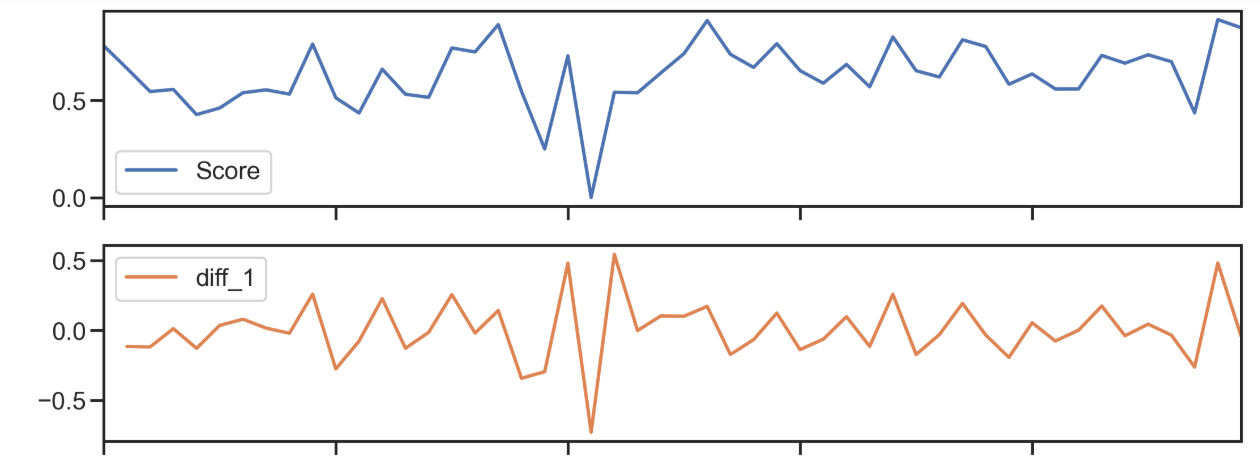
\includegraphics[scale=0.3]{differ.png}
	\caption{The Sequence of First Difference}\label{fig:fig8}
\end{figure}

The original line chart of the score shows that this is an unstable sequence. So we process first difference method on the sequence. Then we get  $p< 0.05$, which means the data passes the test.

We then plot the ACF and PACF of this sequence to select the appropriate p and q of the ARIMA(p, q, d) model. Although there exits an autocorrelation value that exceeds the bounds, we may have p equals 1 due to accidentally exceeding the 95\% confidence interval. Using the same method, according to Figure \ref{fig:fig10}, we can get q equals 1.

\begin{figure}[htbp]
	\centering
	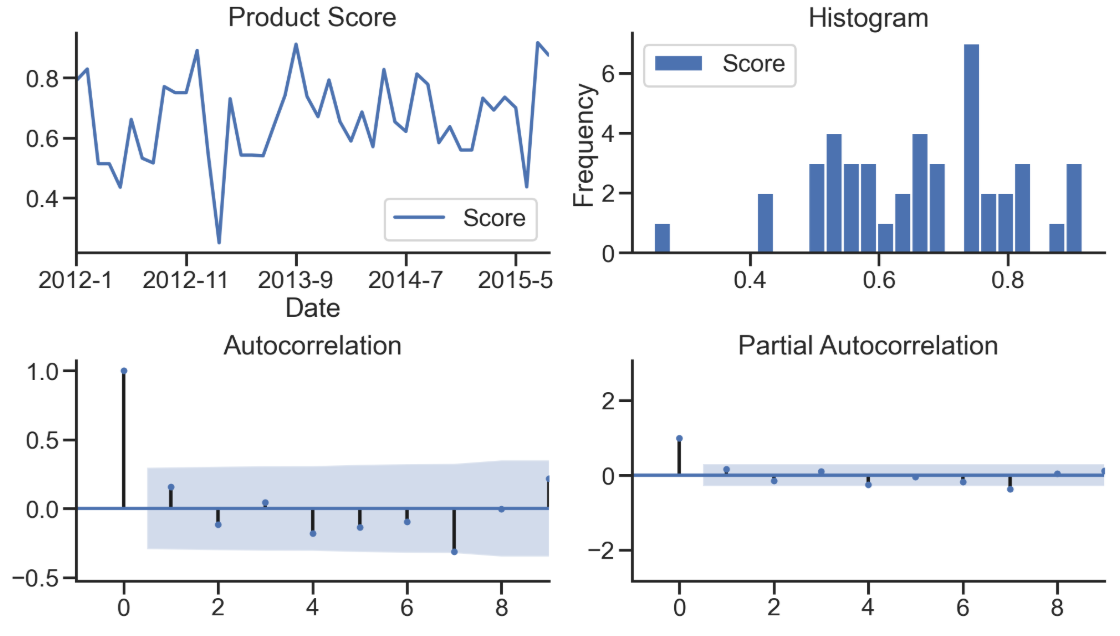
\includegraphics[scale=0.6]{arima.png}
	\caption{ACF and PACF}\label{fig:fig10}
\end{figure}

We use D-W test method to test this model and find it performs well.

\begin{figure}[htbp]
	\centering
	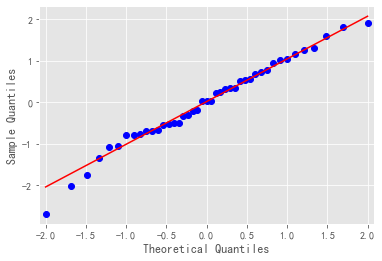
\includegraphics[scale=0.85]{DW.png}
	\caption{The Result D-W Test}\label{fig:fig11}
\end{figure}

Then we can observe the obvious changes in the data from the figure, and the corresponding changes in the reputation can also be clearly observed because the reputation and the score mentioned above are linked. From the figure shown below, it can be seen that reputation has a greater possibility of increasing.

\begin{figure}[htbp]
	\centering
	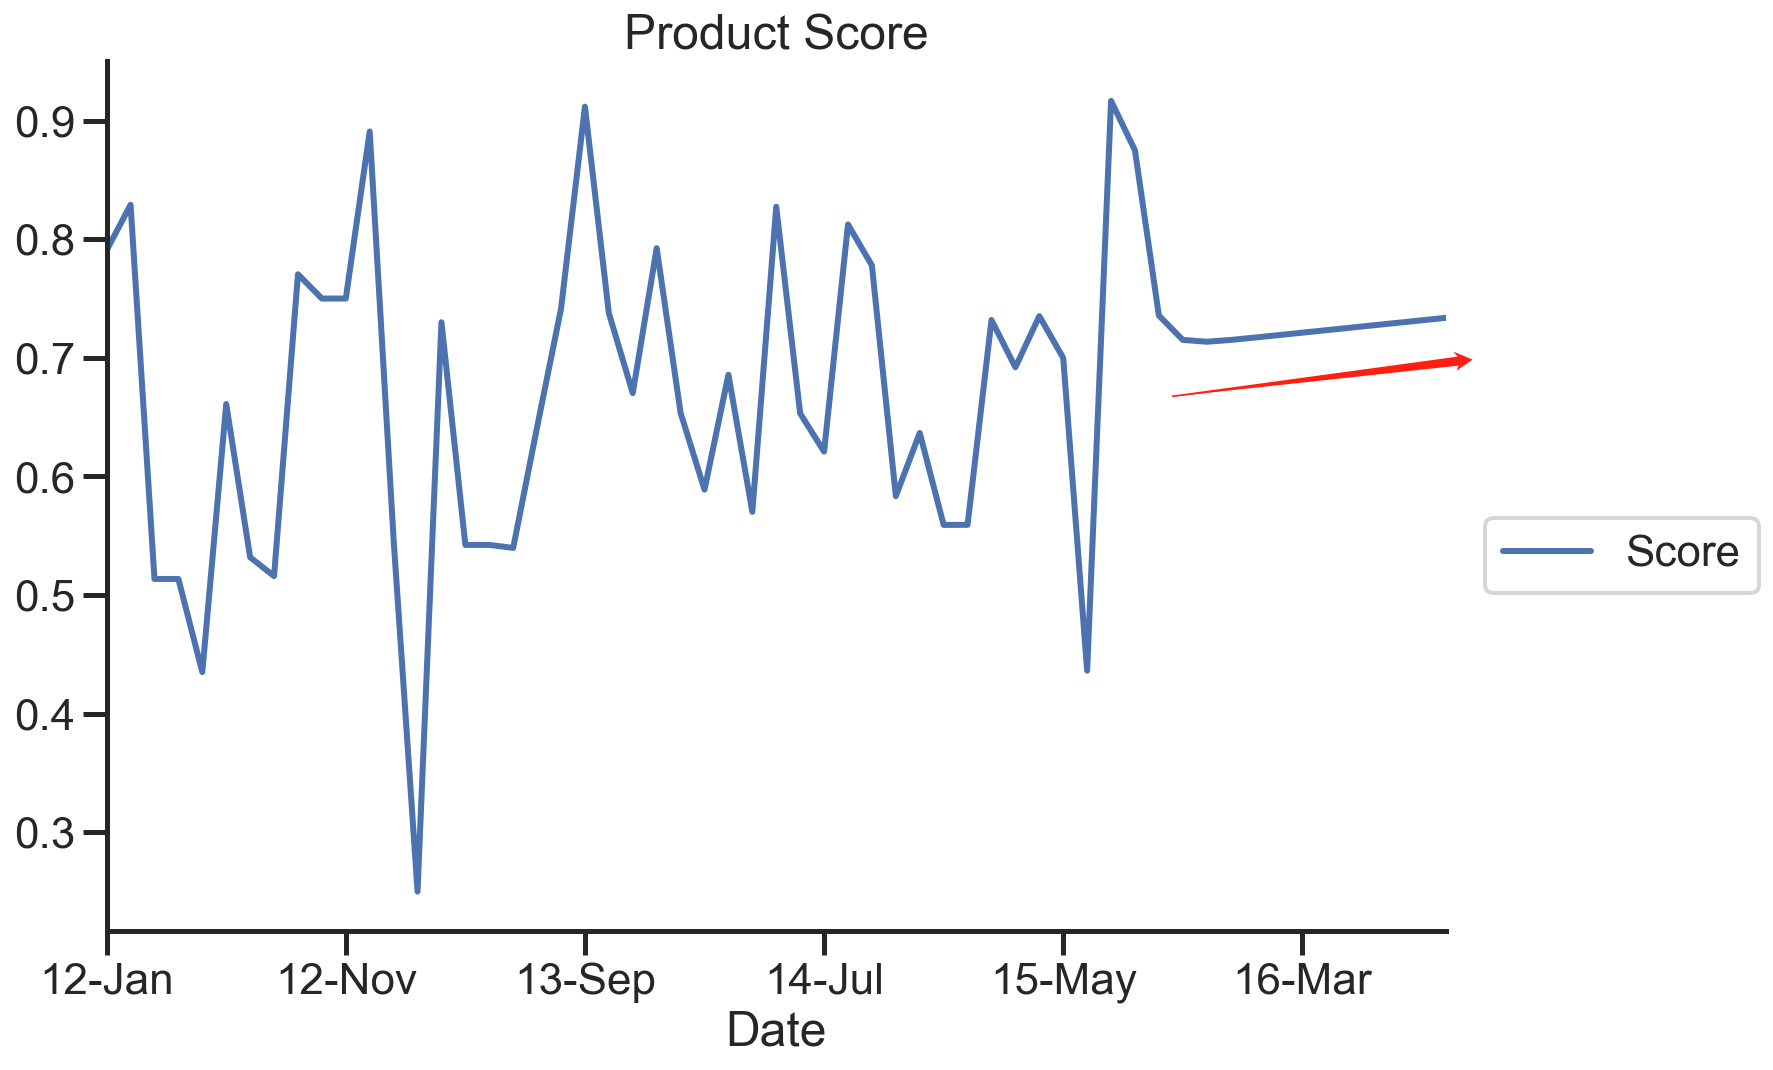
\includegraphics[scale=0.13]{trend.png}
	\caption{The Trend Generated by ARIMA}\label{fig:fig12}
\end{figure} 

\subsection{Non-linear Programming Model}
As we explained in section 4.2, reputation affects the sales of online products. It means that reputation and its change over time conceal information about the quality of the product sales.  Therefore, we map the success or failure of the product to the space of reputation. The base vector of this vector space contains star ratings, review score, helpfulness, etc., and their values range from zero to one. 

We use a non-linear programming model to explore the combinations of dimensions that best indicate a potentially successful or failing product.

The model can be described as,
\begin{equation}\label{eq:model4.3}
\begin{aligned}
&\begin{cases}
max \quad Total \;Score_{product(i)} = f(star \;rating,review\;score,helpfulness,auth,\alpha)
\\[2ex]min \quad Total \;Score_{product(i)} = f(star \;rating,review\;score,helpfulness,auth,\alpha)
\end{cases}\\[2ex]
&\begin{cases}
0 \leq star\; rating \leq 1\\[2ex]
0 \leq sentiment \leq 1\\[2ex]
0 \leq helpfulness \leq 1\\[2ex]
auth \in A,\; A=\{\omega_1,\omega_2,\omega_3\}\\[2ex]
\sum\limits_{j=1}^{2}\alpha_j=1
\end{cases}
\end{aligned}
\end{equation}

The objective function is iterated through the particle swarm optimization algorithm. The pseudo-code of the algorithm is as follows.

\newpage
\begin{algorithm}
        \caption{GF(4) 3D reconstruction}
        \LinesNumbered
        \KwIn{$\mathcal{X}\in\mathbb{R}^{l_1\times l_2\times l_3},K_c,K_p,R,T$}
        \KwOut{$Coord_{i,j}$}
        \textbf{Initialize} all $GF^{(i,j)}s$

        \For{ each $X_{i_j}^k(N_0\le i\le N_1,M_0\le j\le M_1,k \in (r,g,b))$ }
        {
        $d=\max(|
        \sum_{i=-\epsilon}^\epsilon I(x^k +i,y^k)- \sum_{j=-\epsilon}^\epsilon I(x^k,y^k+j)
        |)$\;
        \If{$d > t$}
        {
        $C_{ij}=-1$
        }\Else{
        $Candidate_{ij}=-3$
        }
        }

        \For{ each $Candidate_{i_j}^k(N_0\le i\le N_1,M_0\le j\le M_1)$ }
        {
        \If {$Candidate_{ij}==-1$}
        {
        $\rho_C=\frac{n\sum_{i=1}^nM_{Ci}M_{Ci'}-\sum_{i=1}^nM_{Ci}\sum_{i=1}^nM_{Ci'}}{\sqrt{n\sum_{i=1}^nM_{Ci}^2-(\sum_{i=1}^nM_{Ci})^2}\sqrt{n\sum_{i=1}^nM_{Ci}'^2-(\sum_{i=1}^nM_{Ci'})^2}}$\;
        \If{$\rho_C>t$}
        {
        $GridPoint_{ij}=-1$
        }
        }
        }

        \For{ each $GridPoint_{i_j}^k(N_0\le i\le N_1,M_0\le j\le M_1)$ }
        {
        $FeaturePoint_{i,j}=BFS(GridPoint_{i,j},FLAG)$\;
        \If{$FeaturePoint_{i,j}==-1$}{
        \If{$\sum_{i=-\epsilon}^\epsilon I(x^k +i,y^k)- \sum_{j=-\epsilon}^\epsilon I(x^k,y^k+j)>0$}
        {
        $FeaturePoint_{i,j}=-1$
        }\Else{
        $FeaturePoint_{i,j}=-2$
        }
        }
        }

        \For{ each $FeaturePoint_{i_j}^k(N_0\le i\le N_1,M_0\le j\le M_1)$ }
        {
        \If{$FeaturePoint_{i,j}\neq-1 \; and \; FeaturePoint_{i,j}\neq-2 $}{
        $s=\sqrt{1-\frac{rg+gb+rb}{r^2+g^2+b^2}}$\;
        $h_r=\frac{2r-g-b}{2\sqrt{(r-g)^2}+(r-b)(g-b)}$\;
        $h_g=\frac{2g-r-b}{2\sqrt{(g-r)^2}+(g-b)(r-b)}$\;
        $h_b=\frac{2b-g-r}{2\sqrt{(b-g)^2}+(b-r)(g-r)}$\;
        $k=s-\sqrt{1-\max(h_r,h_g,h_b)}$
        \If{$k<0.2$}
        {
        $FeaturePoint_{i,j}=0$
        }\Else
        {
        $FeaturePoint_{i,j}=\max(r,g,b)$
        }
        }
        }

        \For{ each $FeaturePoint_{i_j}^k(N_0\le i\le N_1,M_0\le j\le M_1)$ }
        {
        \If{$FeaturePoint_{i,j}==-1 \; or \; FeaturePoint_{i,j}==-2$}
        {
        $(u_1m_{31}^1-m_{11}^1)X_W+(u_1m_{32}^1-m_{12}^1)Y_W+(u_1m_{33}^1-m_{13}^1)Z_W=m_{14}^1-u_1m_{34}^1$\;
        $(v_1m_{31}^1-m_{21}^1)X_W+(v_1m_{32}^1-m_{22}^1)Y_W+(v_1m_{33}^1-m_{23}^1)Z_W=m_{24}^1-v_1m_{34}^1$\;
        $(u_1m_{31}^2-m_{11}^2)X_W+(u_1m_{32}^2-m_{12}^2)Y_W+(u_1m_{33}^2-m_{13}^2)Z_W=m_{14}^2-u_1m_{34}^2$\;
        $Coord_{i,j}=(X_W,Y_W,Z_W)$
        }
        }
\end{algorithm}

After several experiments, we get a pair of combinations.\{star rate : 1,review sentiment : 0.75,helpfulness : 1\} will best indicate the  potentially successful product. While \{star rate : 0,review sentiment : 0.5,helpfulness: 0.75\} will best indicate the  potentially failing product.


\subsection{Customer Decision Model}

To investigate the causal relationship between star ratings and reviews, we seek inspiration from social psychology. Hovland Persuasion Model is one of the most classic models in this field. The basic model of this approach can be described as ``who said what to whom'': the source of the communication, the nature of the communication and the nature of the audience\cite{social2010}.
\begin{figure}[h]
	\centering
	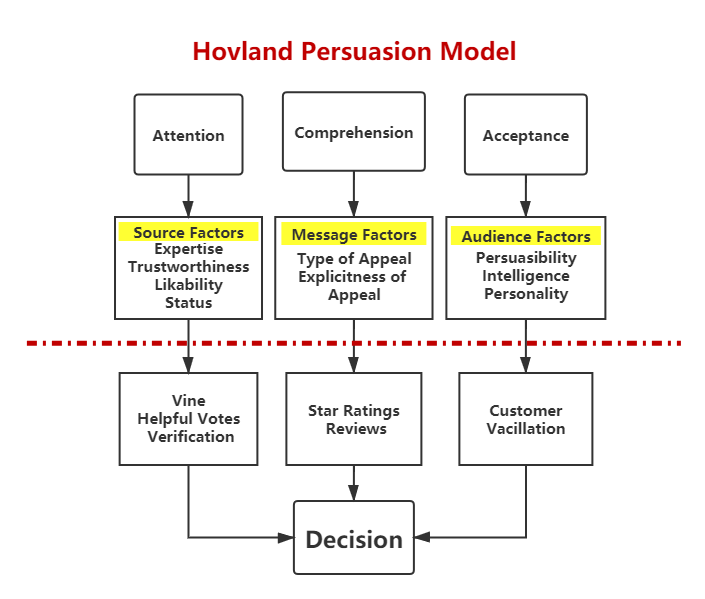
\includegraphics[scale=0.5]{hovland.png}
	\caption{Hovland Persuasion Model Into Practice}\label{fig:fig13}
\end{figure} 

\subsection{Correlation Between Emotional Descriptors and Star Rating}

To analyze specific quality descriptors, we classify all into eight categories using the NRC Emotion Lexicon, including anger, fear, trust, etc. 
The Sentiment and Emotion Lexicons is a collection of lexicons that was entirely created by the experts of the National Research Council of Canada\cite{sentiment.nrc.ca}.

We then use the microwave dataset and find the sentiment distribution of all reviews. As the picture shows, the distribution of review headlines and review bodies is similar across all reviews. Words with emotions like anticipation, trust, and joy, make up the majority. 

\begin{figure}[htbp]
	\centering
	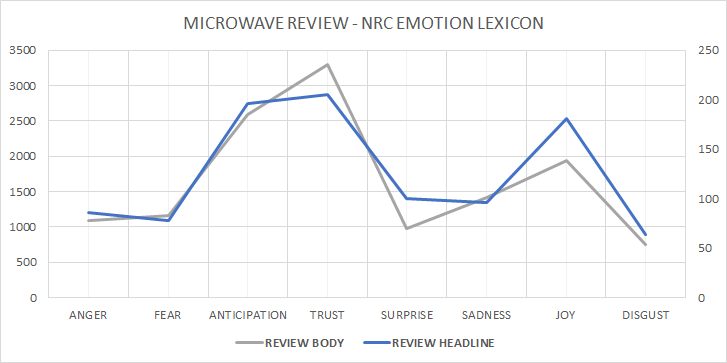
\includegraphics[scale=0.7]{NRCTOTAL.png}
	\caption{Microwave Review - NRC Emotion Lexicon }\label{fig:fig14}
\end{figure}

Generally speaking, in the bad reviews, customers can describe the expectations of the product, but there will not be too many negative descriptions in the good reviews. Therefore, negative descriptions were the focus of our attention.

We match the emotional intensity of eight categories with star ratings to see if they were somehow related. In the eight tables below, the left and right four show the relationship between the intensity of positive emotions and negative emotions and star ratings, respectively. The bars of each colour represent the frequency of that emotional intensity in each star rating level.

\begin{figure}[!h]
	\centering
	\begin{subfigure}[b]{.24\textwidth}
		\centering
		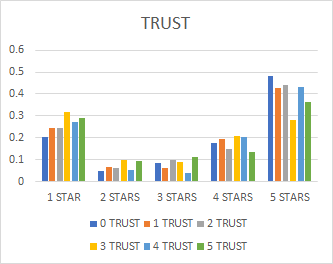
\includegraphics[scale=0.33]{001.png}
		\caption{Trust}
	\end{subfigure}
	\begin{subfigure}[b]{.24\textwidth}
		\centering
		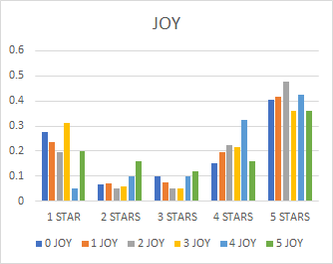
\includegraphics[scale=0.33]{002.png}
		\caption{Joy}
	\end{subfigure}	
	\begin{subfigure}[b]{.24\textwidth}
		\centering
		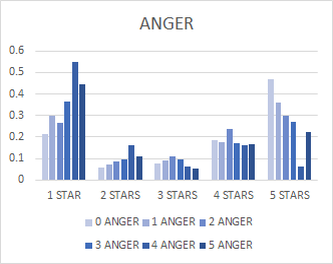
\includegraphics[scale=0.33]{005.png}
		\caption{Anger}
	\end{subfigure}	
	\begin{subfigure}[b]{.24\textwidth}
		\centering
		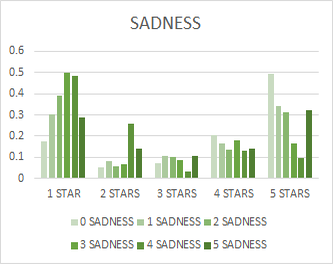
\includegraphics[scale=0.33]{006.png}
		\caption{Sadness}
	\end{subfigure}	
	\begin{subfigure}[b]{.24\textwidth}
		\centering
		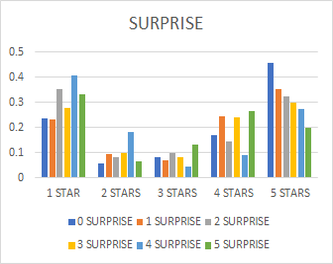
\includegraphics[scale=0.33]{003.png}
		\caption{Surprise}
	\end{subfigure}
	\begin{subfigure}[b]{.24\textwidth}
		\centering
		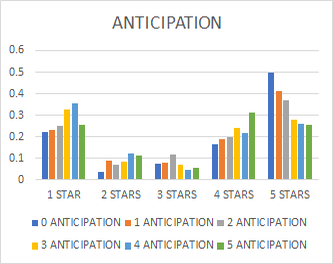
\includegraphics[scale=0.33]{004.png}
		\caption{Anticipation}
	\end{subfigure}	
	\begin{subfigure}[b]{.24\textwidth}
		\centering
		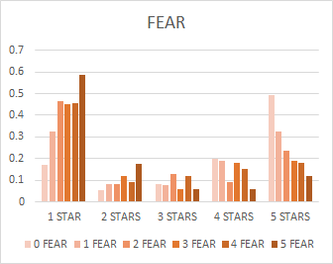
\includegraphics[scale=0.33]{007.png}
		\caption{Fear}
	\end{subfigure}	
	\begin{subfigure}[b]{.24\textwidth}
		\centering
		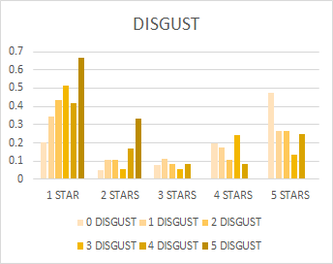
\includegraphics[scale=0.33]{008.png}
		\caption{Disgust}
	\end{subfigure}		
	\caption{Emotional Intensity with Each Star Rating Level}
	\label{fig:logo}
\end{figure}

In a specific star rating, the darker the color of the histogram is, the stronger the emotion of that star rating is. 

In negative emotions, taken 'anger' as an example, reviews with angry words are more found in low stars ratings. Conversely, reviews that did not or rarely contain angry words were more observed in high star ratings. The same goes for the other three negative emotions.

In positive emotions, the distribution ratio of emotional intensity in star ratings is more uniform, especially in low star rating cases.


\section{Sensitivity Analysis}
An essential part of our model is the product measure in section 4.1. In our model, the weight ($\omega_i$) is artificially judged based on experience. Changes in those weights may bring different results. We performed the sensitivity analysis by setting various combinations of weights to see the robustness of our model.

\begin{figure}[htbp]
	\centering
	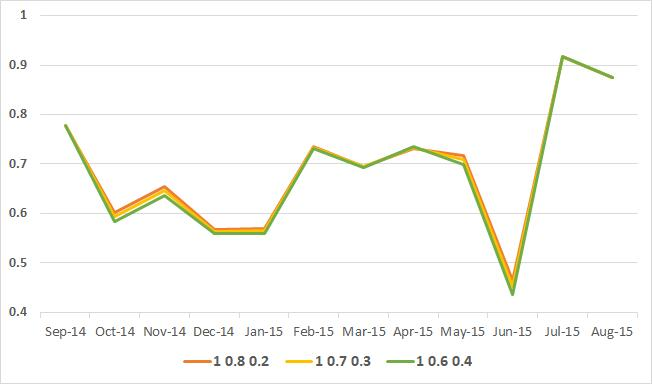
\includegraphics[scale=0.7]{13.jpg}
	\caption{Product.127343313 Total Score }\label{fig:fig15}
\end{figure}

Each of these lines is the product score calculated in a set of given omegas. The green line is the weighted score line we originally designed. As is shown in the figure, when omega changes, the product score is only slightly affected.


\section{Strengths and Weaknesses}
\subsection{Strengths}
\begin{itemize}
    \item We propose a new approach to combine star rating, review and helpfulness rating so that we can quantitatively calculate the overall score of a product and finally integrated them into an evaluation standard.
    
    \item  We perform detailed and fully preprocessing of the review, and we use two different methods to analyze text-based review, including sentiment analysis using SentiWordNet and emotion analysis using NRC Emotion Lexicon.
    
    \item  We have applied the Hovland persuasion model to our model, achieving the combination of the theory of social psychology and real-life context.
    
    \item The model is universal and can be used in other similar scenarios.
    
    \item  We make detailed analysis when determining measures and giving suggestions.
    
    
\end{itemize}

\subsection{Weaknesses}
\begin{itemize}
    \item  In natural language processing, polysemous words such as "right" cannot be classified accurately.
    \item  Misspelling of reviews affects the accuracy of our model.
    
 \end{itemize}


% 以下为信件/备忘录部分,不需要可自行去掉
% 如有需要可将整个 letter 环境移动到文章开头或中间
% 请在后一个花括号内填写信件(Letter)或备忘录(Memorandum)标题
\begin{letter}{Letter}
\begin{flushleft}  % 左对齐环境,无首行缩进
\textbf{To:} Sunshine Company Marketing Director\\
\textbf{From:} Team \#2012050\\
\textbf{Date:} Mar 9th, 2020\\
\textbf{Subject:} Product Review Analysis and Suggestions
\end{flushleft}

Dear Sunshine Company Marketing Director,

After we analyzed the microwave, pacifier and head dryer products sold on Amazon in recent years, we have the following findings and recommendations.

\textbf{Analysis:} Star ratings show customers the quality of the product in an intuitive way. In the existing market on Amazon, the star ratings of microwave ovens indicate a polarized distribution. Reviews reveal customers' concerns. Helpful votes show the quality of a review. With a certain total number of votes, the more helpful votes a review receives from other customers, the more valuable the review is.

\textbf{Measure:} Taken all three main factors into consideration, we provide you with a measure to track. The total score shows the reputation and of a product in a short period.

\textbf{Suggestions:}
~ For those products you have confidence in, invite Amazon Vine to test. Based on Hovland Persuasion Model, vine customers are the most trusted reviewers, so their reviews have more expertise and trustworthiness for other customers and can even affect their reviews.
~ Not only pay attention to the product's ratings, but also the helpful votes. The most helpful reviews will be shown to more potential customers in the 'top review.' 
~ Regularly check the product review, discover the shortcomings of the products proposed by customers, and find the areas that need improvement to upgrade products.

\textbf{Extra Info:} The following are the word clouds for the three product reviews we generated. It is easy to extract the customers' most pressing concerns about the product. For example, for microwave products, customer service and time are the main concerns, which you can improve to increase product competitiveness.

\begin{figure}[h]
	\centering
	\begin{subfigure}[b]{.32\textwidth}
		\centering
		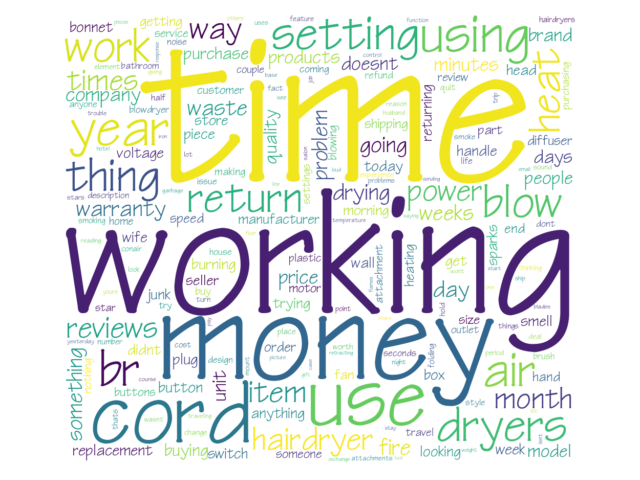
\includegraphics[scale=0.4]{letter_hairdryer.jpg}
		\caption{Review Wordcloud of Hair dryer}
	\end{subfigure}
	\begin{subfigure}[b]{.32\textwidth}
		\centering
		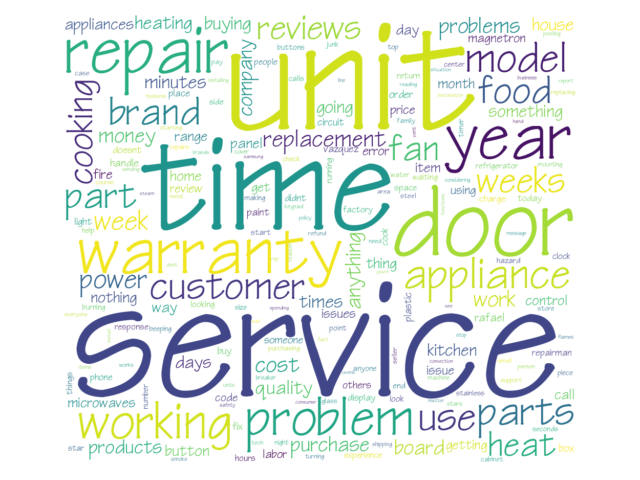
\includegraphics[scale=0.4]{letter_microwave.jpg}
		\caption{Review Worcloud of Microwave}
	\end{subfigure}	
	\begin{subfigure}[b]{.32\textwidth}
		\centering
		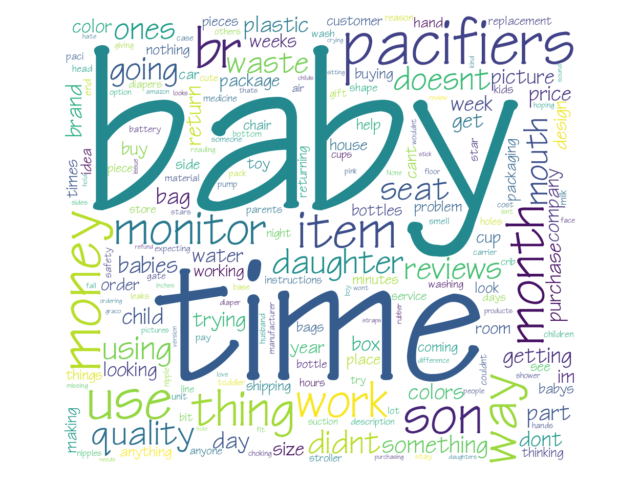
\includegraphics[scale=0.4]{letter_pacifier.jpg}
		\caption{Review Wordcloud of Pacifier}
	\end{subfigure}	
	\caption{Review Wordcloud of Each Product}
	\label{fig:fig16}
\end{figure}


The above is the summary of our study. We sincerely hope that it will provide you with valuable information.
Thanks!

\end{letter}


\bibliography{math}

% 以下为附录内容
% 如您的论文中不需要附录,请自行删除
\begin{subappendices}  % 附录环境

\section{Appendices}
\noindent Here are programmes we used in our model.

\noindent{\color{red}{\textbf{Analyze the sentiment of the review}}}
\lstinputlisting[language=Python,firstline=1,lastline=189]{deal_emotion.py}

\noindent{\color{red}{\textbf{Calculate the score of a single review}}}
\lstinputlisting[language=Python,firstline=1,lastline=216]{cal_score.py}

\noindent{\color{red}{\textbf{NRC Emotion Lexicon: categorize the emotion of a word}}}
\lstinputlisting[language=Python,firstline=1,lastline=97]{nrc.py}



\end{subappendices}

\end{document}  % 结束